\documentclass[10pt,a4paper]{article}

\usepackage[a4paper,margin=2.1cm]{geometry}
\usepackage[T1]{fontenc}
\usepackage{lmodern}
\usepackage{microtype}
\usepackage{amsmath,amssymb}
\usepackage{graphicx}
\usepackage{booktabs}
\usepackage{array}
\usepackage{multirow}
\usepackage{xcolor}
\usepackage{caption}
\usepackage{subcaption}
\usepackage[numbers,sort&compress]{natbib}
\usepackage{tikz}
\usetikzlibrary{positioning,arrows.meta,calc,fit,backgrounds}
\usepackage[colorlinks=true,linkcolor=black,citecolor=black,urlcolor=black]{hyperref}
\usepackage[capitalise,nameinlink]{cleveref}

\captionsetup{font=small,labelfont=bf,skip=4pt}
\setlength{\textfloatsep}{10pt plus 2pt minus 2pt}
\setlength{\floatsep}{8pt plus 2pt minus 2pt}
\setlength{\abovecaptionskip}{3pt}
\setlength{\parskip}{0.25em}

\definecolor{cblue}{HTML}{2a78d6}
\definecolor{corange}{HTML}{eb6834}
\definecolor{caqua}{HTML}{1baf7a}
\definecolor{cgray}{HTML}{52514e}

\newcommand{\pp}{\,pp}

\title{\textbf{Why Neighbour-Consistency Self-Supervision Does Not Help\\Temporal Action Localization:\\A Diagnostic Study with ActionFormer on EPIC-KITCHENS-100}}
\author{[Author name] \\ \small Leiden University \\ \small Master's thesis}
\date{November 2026}

\begin{document}
\maketitle

\begin{abstract}
\noindent
Dense self-supervised objectives such as NeCo, which require the \emph{ordering of
nearest neighbours} of every image patch to agree across augmented views, improve
frozen vision foundation models on semantic segmentation. We ask whether the same
objective, transplanted from 2D image patches to 1D sequences of clip features, improves
temporal action localization (TAL). We adapt NeCo to the multi-scale transformer encoder
of ActionFormer and evaluate it on the EPIC-KITCHENS-100 verb task with SlowFast and
EPIC-finetuned VideoMAE-L features, in two protocols: self-supervised \emph{post}-training
of a converged supervised model, and self-supervised \emph{pre}-training followed by the
full supervised recipe. Post-training lowers average mAP from 23.07 to 21.73. Pre-training
gives no reliable gain: $+0.44$\pp{} over three seeds per arm on SlowFast (Welch
$t\approx1.0$; baseline seed s.d.\ 0.75\pp) and $+0.04$\pp{} on VideoMAE-L. The failure is
not one of optimisation. The SSL objective is fit well (neighbour agreement 0.92--0.94),
and the encoder moves substantially (4--5\% of its weight norm). Instead, the objective
moves the representation in the wrong direction for TAL. A nearest-neighbour probe shows
that NeCo makes timesteps \emph{less} likely to have neighbours with the same verb, both across and
within videos (verb-label lift 0.31$\rightarrow$0.26 on SlowFast). An SSL-initialised
model starts supervised training with a 1--5\% \emph{higher} loss than a randomly
initialised one, and supervised training erases the SSL changes entirely. In NeCo's own
setting (DINOv2 $\rightarrow$ PASCAL VOC), the same three probes all point the other way:
neighbours become more label-consistent, the first-epoch loss is 5--10\% lower, and
linear-probe mIoU rises by 2.0. Two natural explanations do not hold up. The views are
not the cause: temporal crops of pre-extracted features give identical input to 93--97\%
of the finest-level positions, but spatial crops, which differ at every timestep as image
views do, produce the same drop. Nor does NeCo exploit scene identity: it removes kitchen
identity from the neighbourhoods (same-kitchen neighbours 0.50$\rightarrow$0.31) along
with verb identity. What distinguishes our setting from NeCo's is the starting point.
Instead of refining generic features that encode objects, NeCo re-mixes clip features
that were already supervised for the target verbs, and its neighbour-order target does not
coincide with verb identity.
\end{abstract}

%=======================================================================================
\section{Introduction}
%=======================================================================================

Temporal action localization (TAL) asks a model to find \emph{when} each action in an
untrimmed video starts and ends and \emph{what} it is. Modern single-stage detectors such
as ActionFormer~\cite{zhang2022actionformer} operate on pre-extracted clip features: a
frozen video backbone (e.g.\ SlowFast~\cite{feichtenhofer2019slowfast} or
VideoMAE~\cite{tong2022videomae}) turns a video into a sequence of feature vectors, and a
light multi-scale transformer encoder followed by classification and regression heads is
trained on top. The encoder is the only part of this pipeline that learns temporal
context, and it is trained from scratch on a few hundred labelled videos.

Self-supervised learning (SSL) is the standard answer to scarce labels. Among dense SSL
objectives, NeCo~\cite{pariza2025neco} is attractive for localization: rather than making
whole-image embeddings invariant, it asks every patch to rank a set of reference patches
in the same order in two augmented views. Applied as a short post-training stage on
DINOv2~\cite{oquab2024dinov2}, it gives consistent gains on semantic segmentation. The
ActionFormer encoder is structurally a dense per-timestep feature extractor over a 1D
sequence, so the analogy is direct: temporal positions play the role of patches, and
temporal crops the role of image crops. If neighbourhood consistency helps patches find
the right semantic neighbours, it might help timesteps find the right action neighbours.

This thesis tests that analogy and reports a negative result: \textbf{NeCo-style SSL does
not improve ActionFormer on EPIC-KITCHENS-100 verbs}, neither as post-training nor as
pre-training. Negative results are only useful if their cause is understood, so most of
the work goes into the diagnosis. Our contributions are:
\begin{itemize}\setlength\itemsep{0pt}
\item A 1D adaptation of NeCo to ActionFormer's encoder (temporal and spatial crops,
  multi-scale 1D ROI-Align, cross-video teacher references, an EMA teacher), and a
  transfer path that plugs the SSL encoder into the unmodified supervised recipe
  (\cref{sec:method}).
\item A controlled evaluation of post-training and pre-training on SlowFast and
  VideoMAE-L features, with seed replicates for the main comparison (\cref{sec:results}).
\item A diagnosis that rules out the optimisation explanations (the objective is fit and
  the encoder moves) and shows instead that NeCo pushes timestep neighbourhoods
  \emph{away} from the verb structure. We separate the contributions of views, starting
  representation and scene identity (\cref{sec:why}).
\item A positive control in NeCo's own setting, using the same three probes. There they
  all point the other way, which localises the failure to the TAL setting rather than to
  the objective (\cref{sec:voc}).
\end{itemize}

%=======================================================================================
\section{Related Work}
%=======================================================================================

\paragraph{Temporal action localization.}
Early proposal-based methods such as BMN~\cite{lin2019bmn} and
G-TAD~\cite{xu2020gtad} were overtaken by single-stage transformer detectors.
ActionFormer~\cite{zhang2022actionformer} combines a convolutional embedding, a
multi-scale transformer with local self-attention, and per-timestep classification and
boundary regression heads. TriDet~\cite{shi2023tridet} and many later methods keep this
backbone and change the heads. Nearly all of these operate on frozen features, and much
of the recent progress has come from better features (e.g.\ EPIC-finetuned VideoMAE) or
from end-to-end backbone adaptation~\cite{liu2024adatad,liu2025opentad}.

\paragraph{Self-supervised dense representation learning.}
Joint-embedding SSL learns invariances to the augmentations used to create
views~\cite{chen2020simclr,grill2020byol,caron2021dino}. Which invariances are learned is
determined almost entirely by how the views differ~\cite{tian2020goodviews}. Dense
variants transfer this idea from images to patches. Leopart~\cite{ziegler2022leopart}
clusters patch features, and NeCo~\cite{pariza2025neco} replaces patch-to-prototype
matching with a differentiable sort~\cite{prillo2020softsort} of patch-to-reference
distances, aligning the two views with ROI-Align~\cite{he2017maskrcnn} and using an EMA
teacher~\cite{tarvainen2017meanteacher}.

\paragraph{Pre-training for localization.}
Localization-specific pre-training of the \emph{video backbone}, such as
TSP~\cite{alwassel2021tsp} and BSP~\cite{xu2021bsp}, improves TAL by changing the features
themselves. Our setting is different: the backbone and its features are fixed, and only
the TAL encoder on top is pre-trained. Results from image recognition suggest caution.
He et al.~\cite{he2019rethinking} found that with a full training schedule, ImageNet
pre-training mainly speeds up convergence rather than improving final accuracy, and Raghu
et al.~\cite{raghu2019transfusion} found that much of what transfer provides is weight
scaling rather than reusable features. We measure the analogous quantities directly.

%=======================================================================================
\section{Method}\label{sec:method}
%=======================================================================================

\subsection{ActionFormer}
A video is represented by a sequence of frozen clip features $X\in\mathbb{R}^{T\times C}$
(SlowFast: $C{=}2304$, one vector every 16 frames at 30\,fps, i.e.\ 1.875 vectors/s).
The encoder $f_\theta$ consists of two 1D convolutions (kernel 3), two transformer blocks,
and five further transformer blocks that each halve the temporal resolution, producing a
six-level feature pyramid $\{F^{(l)}\}_{l=0}^{5}$ with stride $2^l$ and 512 channels. All
self-attention is local, with a window of 9 positions. An identity neck passes the pyramid to
shared classification and regression heads, trained with focal~\cite{lin2017focal} and
DIoU~\cite{zheng2020diou} losses and center sampling. At inference,
Soft-NMS~\cite{bodla2017softnms} merges candidates from all levels. The encoder
(``backbone + neck'', 207 parameter tensors) is shared by every protocol below; only the
heads differ.

\subsection{NeCo on a temporal feature sequence}\label{sec:neco1d}

\begin{figure}[t]
\centering
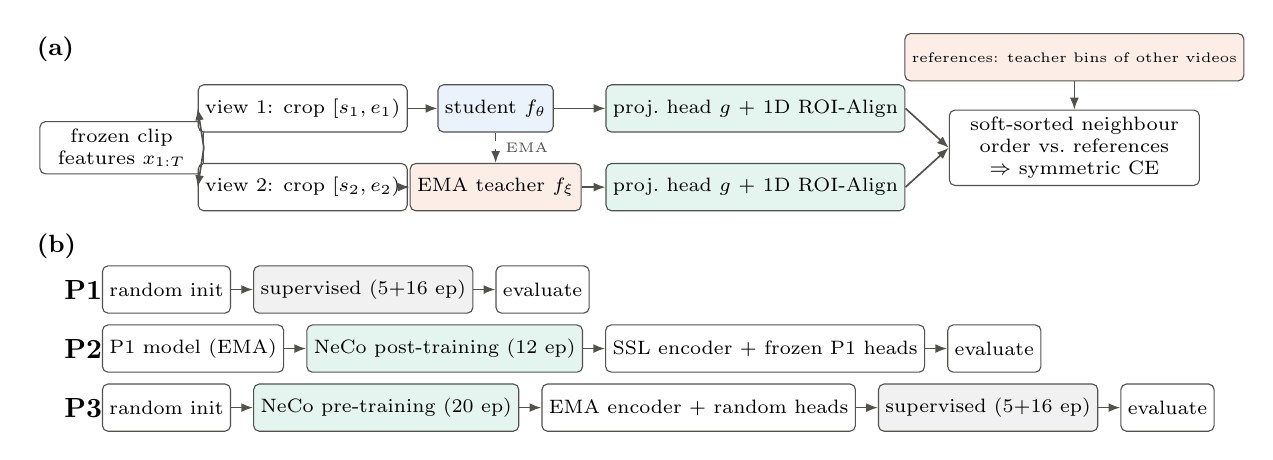
\begin{tikzpicture}[font=\scriptsize,
  box/.style={draw=cgray, rounded corners=2pt, align=center, inner sep=2.5pt, minimum height=0.6cm, fill=white},
  sbox/.style={box, fill=cblue!10}, tbox/.style={box, fill=corange!12}, hbox/.style={box, fill=caqua!12},
  arr/.style={-{Latex[length=1.5mm]}, semithick, cgray}]
% ---------------- (a) objective
\node[font=\small\bfseries, anchor=west] at (-0.2, 0.75) {(a)};
\node[box, text width=1.9cm] (x) at (1.0,-0.5) {frozen clip features $x_{1:T}$};
\node[box] (v1) at (3.3, 0.0) {view 1: crop $[s_1,e_1)$};
\node[box] (v2) at (3.3,-1.0) {view 2: crop $[s_2,e_2)$};
\node[sbox] (s) at (5.75, 0.0) {student $f_\theta$};
\node[tbox] (t) at (5.75,-1.0) {EMA teacher $f_\xi$};
\node[hbox] (g1) at (9.05, 0.0) {proj.\ head $g$ + 1D ROI-Align};
\node[hbox] (g2) at (9.05,-1.0) {proj.\ head $g$ + 1D ROI-Align};
\node[box, text width=3.0cm] (L) at (13.1,-0.5) {soft-sorted neighbour\\order vs.\ references\\$\Rightarrow$ symmetric CE};
\node[box, font=\tiny, fill=corange!12] (R) at (13.1, 0.65) {references: teacher bins of other videos};
\draw[arr] (x.east) -- (v1.west); \draw[arr] (x.east) -- (v2.west);
\draw[arr] (v1) -- (s); \draw[arr] (v2) -- (t);
\draw[arr] (s) -- (g1); \draw[arr] (t) -- (g2);
\draw[arr] (g1.east) -- (L.west); \draw[arr] (g2.east) -- (L.west); \draw[arr] (R) -- (L);
\draw[arr, dashed] (s) -- node[right, font=\tiny]{EMA} (t);
% ---------------- (b) protocols
\node[font=\small\bfseries, anchor=west] at (-0.2,-1.75) {(b)};
\def\gap{0.28cm}
\node[font=\bfseries, anchor=west] at (0.15,-2.3) {P1};
\node[box, anchor=west] (p1a) at (0.75,-2.3) {random init};
\node[box, right=\gap of p1a, fill=cgray!8] (p1b) {supervised (5+16 ep)};
\node[box, right=\gap of p1b] (p1c) {evaluate};
\draw[arr] (p1a) -- (p1b); \draw[arr] (p1b) -- (p1c);
\node[font=\bfseries, anchor=west] at (0.15,-3.05) {P2};
\node[box, anchor=west] (p2a) at (0.75,-3.05) {P1 model (EMA)};
\node[box, right=\gap of p2a, fill=caqua!12] (p2b) {NeCo post-training (12 ep)};
\node[box, right=\gap of p2b] (p2c) {SSL encoder + frozen P1 heads};
\node[box, right=\gap of p2c] (p2d) {evaluate};
\draw[arr] (p2a) -- (p2b); \draw[arr] (p2b) -- (p2c); \draw[arr] (p2c) -- (p2d);
\node[font=\bfseries, anchor=west] at (0.15,-3.8) {P3};
\node[box, anchor=west] (p3a) at (0.75,-3.8) {random init};
\node[box, right=\gap of p3a, fill=caqua!12] (p3b) {NeCo pre-training (20 ep)};
\node[box, right=\gap of p3b] (p3c) {EMA encoder + random heads};
\node[box, right=\gap of p3c, fill=cgray!8] (p3d) {supervised (5+16 ep)};
\node[box, right=\gap of p3d] (p3e) {evaluate};
\draw[arr] (p3a) -- (p3b); \draw[arr] (p3b) -- (p3c); \draw[arr] (p3c) -- (p3d); \draw[arr] (p3d) -- (p3e);
\end{tikzpicture}
\caption{\textbf{(a)} NeCo adapted to 1D. Two overlapping crops of the same pre-extracted
feature sequence are encoded by a student and an EMA teacher. Every pyramid level is
projected and ROI-aligned onto the crop intersection, and the loss asks the ordering of
reference bins (teacher features of the other videos in the batch) to agree between the
two views. \textbf{(b)} The three protocols. P1 is the supervised baseline. P2 post-trains
the encoder of a converged P1 model and splices it back onto the frozen P1 heads. P3
runs SSL from a random initialisation and transfers the EMA encoder into the
unmodified supervised recipe, so only the encoder's starting point differs from P1.}
\label{fig:method}
\end{figure}

\paragraph{Views.} Following NeCo, each training sample yields two views, but here they
are crops of a 1D sequence (\cref{fig:method}a). For a video of $T$ feature steps
(randomly windowed to the encoder's maximum length if longer), two crop lengths are drawn
uniformly from $[\max(0.4T, 128), T]$, and the crops are placed so that they overlap by at
least 20\% of the shorter one. Their intersection $[\max(s_1,s_2), \min(e_1,e_2))$ is the
shared region of interest (ROI). The student encodes view~1 and the teacher view~2. As a
second view type for VideoMAE-L we use \emph{spatial crops}: 16 spatial crops per snippet
are extracted from the backbone's dense tokens and pooled. The two views then cover the
same time span but see different image regions, so they differ in their input at every
timestep.

\paragraph{Projection and alignment.} At every pyramid level, a 3-layer position-wise MLP
$g$ (512$\to$2048$\to$2048$\to$256, GELU, dropout 0.1) projects the features. A 1D
ROI-Align then linearly interpolates them at $N{=}32$ equally spaced bin centres in
the ROI, expressed in each view's own coordinates and the level's stride. The six aligned
levels are concatenated, fused by a linear mixer with LayerNorm, and L2-normalised, giving
anchors $z^{s}_{b,n}$ (student) and $z^{t}_{b,n}$ (teacher) for video $b$ and bin $n$.

\paragraph{Neighbour-order loss.} As in NeCo, references come from the teacher. For video
$b$, the reference set $O_b=\{o_r\}_{r=1}^{R}$ contains a random half of the valid
\emph{teacher} bins of every other video in the batch ($R=48$ for batch size 4). With
distances $d^{v}_{n,r}=-\langle z^{v}_{b,n}, o_r\rangle$ for $v\in\{s,t\}$,
SoftSort~\cite{prillo2020softsort} gives a differentiable rank
$\rho^{v}_{n,r}=\sum_{j}\sigma\big((d^{v}_{n,r}-d^{v}_{n,j})/\tau_r\big)$ and a soft
permutation matrix
\begin{equation}
P^{v}_{n}[k,r]=\operatorname{softmax}_r\!\Big(-\frac{|k-\rho^{v}_{n,r}|}{\tau_p}\Big),
\qquad k=0,\dots,R-1,
\end{equation}
i.e.\ the probability that reference $r$ is the $k$-th nearest neighbour of anchor $n$.
The loss is the symmetric cross-entropy between the two views' soft permutations,
\begin{equation}
\mathcal{L}_{\text{NeCo}}=\frac{1}{|\mathcal{A}|}\sum_{(b,n)\in\mathcal{A}}\frac{1}{R}
\Big[\operatorname{CE}\big(P^{t}_{n},P^{s}_{n}\big)+\operatorname{CE}\big(P^{s}_{n},P^{t}_{n}\big)\Big],
\quad \operatorname{CE}(P,Q)=-\sum_{k,r}P[k,r]\log Q[k,r],
\end{equation}
with $\tau_r=\tau_p=0.1$. We also log the \emph{top-1 agreement}: the fraction of anchors
whose nearest reference is the same in both views. The teacher is an exponential moving
average $\xi\leftarrow m\,\xi+(1-m)\,\theta$ whose momentum follows a cosine schedule
from $m_0=0.99$ to 1. Its time constant ($\sim$100 steps) is short compared with the runs
(1476--2460 steps), so the teacher tracks the student and the transferred encoder carries
the SSL training.

\subsection{Protocols}
\Cref{fig:method}b summarises the three protocols. \textbf{P1} is the supervised
baseline. \textbf{P2 (post-training)} follows NeCo's own use case. It starts from the
converged P1 model (its EMA weights, i.e.\ the evaluated model), trains the encoder with
$\mathcal{L}_{\text{NeCo}}$ using NeCo's post-training recipe (small encoder learning rate,
10$\times$ larger head learning rate), and evaluates the EMA encoder spliced onto the
frozen P1 heads. \textbf{P3 (pre-training)}, the order used in the SSL literature, runs
$\mathcal{L}_{\text{NeCo}}$ from a random initialisation (stage~A). It then loads only the
backbone and neck from the SSL checkpoint's EMA teacher and trains the whole model with
the unmodified P1 recipe (stage~B). Because stage~A trains from scratch, it uses a
from-scratch recipe: the supervised learning rate for the encoder, no head multiplier, and
20 epochs. \Cref{sec:results} shows that the post-training recipe is too gentle for this.

%=======================================================================================
\section{Experimental Setup}\label{sec:setup}
%=======================================================================================

\paragraph{Data and features.} EPIC-KITCHENS-100~\cite{damen2022epic}, verb task
(97 classes): 495 training and 138 validation videos of egocentric kitchen activity
(the validation videos come from 32 kitchens); we evaluate on the validation split. We use
\textbf{SlowFast}, the official EPIC-pretrained features used by ActionFormer (2304-d,
32-frame windows, stride 16), and \textbf{VideoMAE-L} fine-tuned on EPIC verbs, as released
by OpenTAD~\cite{liu2025opentad} (1024-d, 16-frame windows, stride 8). As a feature-quality
reference we also train the supervised baseline on frozen
\textbf{V-JEPA~2}~\cite{assran2025vjepa2} ViT-L features, which are not adapted to EPIC.

\paragraph{Training.} \Cref{tab:hparams} lists the schedules. Supervised training is the
published ActionFormer recipe and is identical in P1 and P3 stage~B.

\begin{table}[t]
\centering\small
\caption{Training schedules. One SSL epoch is 123 iterations (batch 4). All SSL runs use
teacher references and an EMA teacher with momentum $0.99\rightarrow1$.}
\label{tab:hparams}
\begin{tabular}{lccc}
\toprule
 & Supervised (P1, P3-B) & SSL post-training (P2) & SSL pre-training (P3-A) \\
\midrule
starting point & random & P1 model (EMA) & random \\
epochs (warm-up + main) & 5 + 16 & 2 + 10 & 2 + 18 \\
optimizer, batch size & AdamW, 2 & AdamW, 4 & AdamW, 4 \\
encoder learning rate & $1{\times}10^{-4}$ & $2{\times}10^{-5}$ & $1{\times}10^{-4}$ \\
head learning rate & $1{\times}10^{-4}$ & $2{\times}10^{-4}$ (10$\times$) & $1{\times}10^{-4}$ (1$\times$) \\
grad.\ clip (global L2) & 1.0 & 1.0 & 5.0 \\
\bottomrule
\end{tabular}
\end{table}

\paragraph{Evaluation and statistics.} We report mAP at temporal IoU
$\{0.1,\dots,0.5\}$ and their average (``avg mAP''), from the EMA model after the final
epoch. The main comparison (SlowFast P1 vs.\ P3) uses three seeds per arm; for P3, both
stages are re-seeded. Other rows are single runs. We use the SlowFast baseline's seed
standard deviation (0.75\pp) as the noise scale for single-run differences.

\paragraph{Diagnostics.} \emph{Weight movement} is
$\|W-W_0\|_2/\|W_0\|_2$ over all backbone weights, where $W_0$ is the starting point. The
\emph{neighbour-label probe} is the TAL counterpart of NeCo's patch-neighbour analysis:
for each foreground validation timestep (up to 20k), we take the 10 cosine nearest
neighbours of its level-0 encoder feature, either from other videos or from the same video
outside a $\pm$16-step window (8.5\,s), and measure how often a neighbour shares one of its
verb labels. We report \emph{lift over chance}, $(a-c)/(1-c)$, where $c$ is the same
fraction over all candidates. The \emph{kitchen probe} measures how often the cross-video
neighbours come from the same participant's kitchen. The \emph{head-start probe} compares
the first-epoch supervised loss of seed-matched SSL-initialised and randomly initialised
runs, which share the head initialisation and data order.

%=======================================================================================
\section{Results}\label{sec:results}
%=======================================================================================

\begin{table}[t]
\centering\small
\caption{EPIC-KITCHENS-100 verb, validation mAP (\%). Mean $\pm$ sample s.d.\ where $n{=}3$;
other rows are single runs. P2 is compared with the model it starts from (P1, seed 0).}
\label{tab:main}
\setlength{\tabcolsep}{5pt}
\begin{tabular}{llcccccc}
\toprule
Features & Model & 0.1 & 0.2 & 0.3 & 0.4 & 0.5 & Avg \\
\midrule
\multirow{6}{*}{SlowFast}
 & ActionFormer (paper~\cite{zhang2022actionformer}) & 26.6 & 25.4 & 24.2 & 22.3 & 19.1 & 23.5 \\
 & P1 baseline ($n{=}3$) & 26.67 & 25.51 & 24.16 & 21.98 & 18.58 & 23.38\,$\pm$\,0.75 \\
 & \quad P1, seed 0 (start of P2) & 26.40 & 25.15 & 23.73 & 21.70 & 18.35 & 23.07 \\
 & P2 post-training, frozen heads & 25.05 & 24.05 & 22.49 & 20.07 & 17.01 & 21.73 \\
 & P3 pre-training ($n{=}3$) & 26.89 & 25.96 & 24.38 & 22.59 & 19.27 & 23.82\,$\pm$\,0.18 \\
 & P3 with the post-training SSL recipe & 26.78 & 25.39 & 23.92 & 22.07 & 18.67 & 23.37 \\
\midrule
\multirow{3}{*}{VideoMAE-L}
 & P1 baseline & 32.84 & 32.06 & 30.42 & 28.11 & 24.59 & 29.60 \\
 & P3, temporal crops & 32.90 & 32.25 & 30.38 & 28.12 & 24.54 & 29.64 \\
 & P3, spatial crops & 32.48 & 31.78 & 30.20 & 27.85 & 23.77 & 29.22 \\
\midrule
V-JEPA 2 & P1 baseline & 20.51 & 19.74 & 18.38 & 16.17 & 12.64 & 17.49 \\
\bottomrule
\end{tabular}
\end{table}

\begin{figure}[t]
\centering
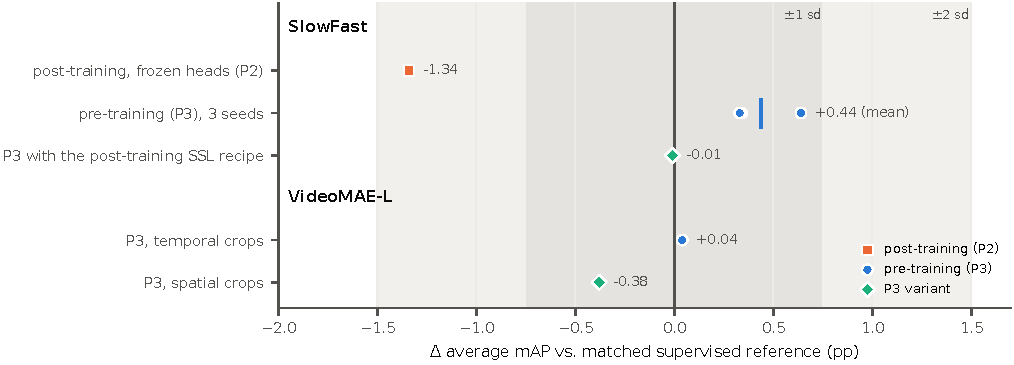
\includegraphics[width=\linewidth]{figs/fig_results.pdf}
\caption{Every SSL variant as a difference in average mAP to its matched supervised
reference. Shaded bands: $\pm1$ and $\pm2$ standard deviations of the SlowFast baseline
over seeds (0.75\pp), the only measured noise scale, applied to all rows. Post-training
falls well below its reference; no pre-training variant leaves the $\pm1$\,s.d.\ band.}
\label{fig:results}
\end{figure}

\Cref{tab:main} gives all results, and \cref{fig:results} shows each variant against its
reference. Our SlowFast reproduction (23.38\,$\pm$\,0.75 over three seeds; range
22.84--24.23) brackets the published 23.5. Feature choice dominates everything else:
VideoMAE-L is 6.2\pp{} above SlowFast and 12.1\pp{} above frozen V-JEPA~2, an order of
magnitude more than any SSL effect.

\paragraph{Post-training hurts.} P2 lowers SlowFast from 23.07 to 21.73 ($-1.34$\pp), at
every tIoU threshold. The SSL objective itself is fit well (top-1 agreement
$0.70\rightarrow0.93$), and the encoder moves only 0.87\% from the supervised weights it
started from. \Cref{sec:why-knn} shows that this small update leaves the encoder's verb
neighbourhoods intact but shifts the features away from what the frozen heads were
trained on.

\paragraph{Pre-training does not raise mAP.} SlowFast P3 reaches 23.82\,$\pm$\,0.18 against
23.38\,$\pm$\,0.75 for the baseline: $+0.44$\pp, Welch $t\approx1.0$ ($p\approx0.4$). The
seed-matched differences ($+0.95$, $+0.88$, $-0.52$) mostly reflect the spread of the
baseline seeds. The best single run is a baseline seed (24.23). On VideoMAE-L, P3 matches the
baseline to within 0.2\pp{} at every threshold (29.64 vs.\ 29.60). With spatial-crop views
it reaches 29.22 ($-0.38$\pp, within one seed s.d.).

\paragraph{The SSL recipe determines whether the encoder trains.} Running stage~A with
NeCo's post-training recipe instead of the from-scratch recipe moves the encoder by only
0.43\% (\cref{sec:why-trains}). The result is indistinguishable from the baseline (23.37),
because the transferred encoder is still essentially the random initialisation. All other
P3 results use the from-scratch recipe, under which the encoder moves by 4--5\%.

\begin{figure}[t]
\centering
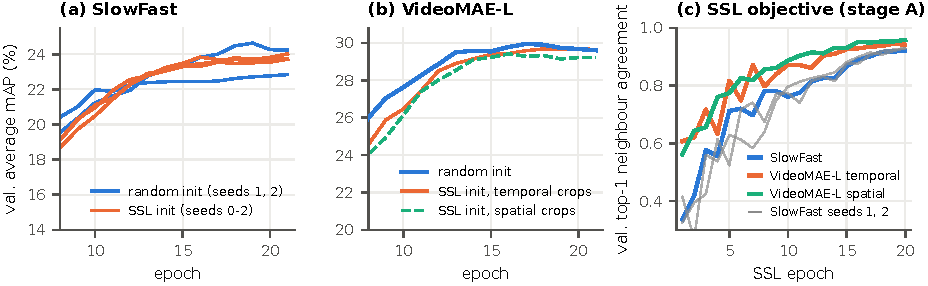
\includegraphics[width=\linewidth]{figs/fig_trajectories.pdf}
\caption{\textbf{(a, b)} Validation average mAP during supervised training from a random
(blue) and an SSL-initialised (orange) encoder. The curves overlap from epoch 10 on, and
the seed spread (a) is as large as any gap between the arms. \textbf{(c)} The SSL
objective during stage A: top-1 neighbour agreement on the validation split rises to
0.92--0.94 in every run.}
\label{fig:trajectories}
\end{figure}

%=======================================================================================
\section{Why NeCo Does Not Help}\label{sec:why}
%=======================================================================================

The obvious explanations for a null SSL result are that the objective was not optimised,
or that the encoder did not change. \Cref{sec:why-trains} rules both out. The rest of the
section shows that the objective changes the representation in a direction that is
useless or harmful for TAL (\cref{sec:why-knn,sec:why-erase}), examines why
(\cref{sec:why-views,sec:why-scene}), and contrasts all of it with NeCo's own setting
(\cref{sec:voc}).

\subsection{An upper bound: SSL cannot add information}\label{sec:why-info}
The clip features are computed once by a frozen backbone and are identical in every run.
SSL and supervised training see exactly the same tensors from exactly the same 495 videos.
By the data-processing inequality~\cite{cover2006elements}, no function of those tensors
contains more information about the actions than the tensors themselves. The SSL stage
can only change \emph{where the encoder starts} when it learns to combine a fixed
representation. For features already fine-tuned on EPIC verbs (VideoMAE-L) or pre-trained
on EPIC (SlowFast), that representation already carries the verb structure. This bounds
the achievable gain but does not predict zero: a better starting point could still help
optimisation or generalisation.

\subsection{The SSL stage trains the encoder}\label{sec:why-trains}

\begin{figure}[t]
\centering
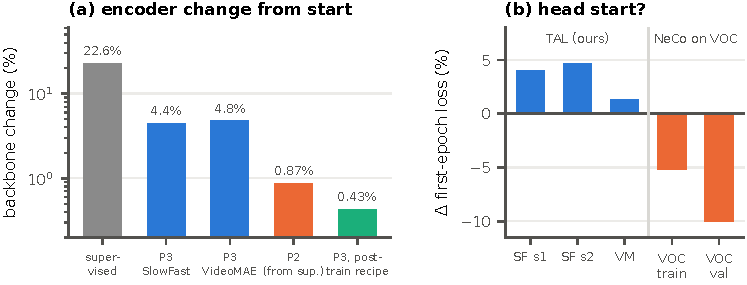
\includegraphics[width=0.84\linewidth]{figs/fig_movement.pdf}
\caption{\textbf{(a)} Change of the transferred backbone weights relative to their
starting point (log scale). P3 stage A moves the encoder by 4--5\%, a fifth of what full
supervised training does. P2 moves the supervised encoder by 0.87\%. With NeCo's
post-training recipe, a from-scratch stage A moves it by only 0.43\%. \textbf{(b)}
Head-start probe: first-epoch supervised loss of SSL-initialised minus randomly
initialised runs with identical head initialisation and data order. In TAL the
SSL-initialised model starts \emph{worse}. In NeCo's own setting it starts better.}
\label{fig:movement}
\end{figure}

Stage~A fits the NeCo objective in every run. The validation loss falls from 13--19 to
1.1--1.6, and the top-1 neighbour agreement rises to 0.92 (SlowFast) and 0.94
(VideoMAE-L; \cref{fig:trajectories}c). The fit also reaches the transferred weights. The
EMA teacher's backbone moves by 4.4\% (SlowFast) and 4.8\% (VideoMAE-L) from its random
initialisation, within 3\% of the student's movement, and the projection head by 8--9\%
(\cref{fig:movement}a). Full supervised training moves the same backbone by 23\%, so the
SSL stage makes a change one fifth the size of training the detector itself. The null
result is therefore not one of an encoder that SSL failed to train.

\subsection{NeCo moves timestep neighbourhoods away from verbs}\label{sec:why-knn}

\begin{figure}[t]
\centering
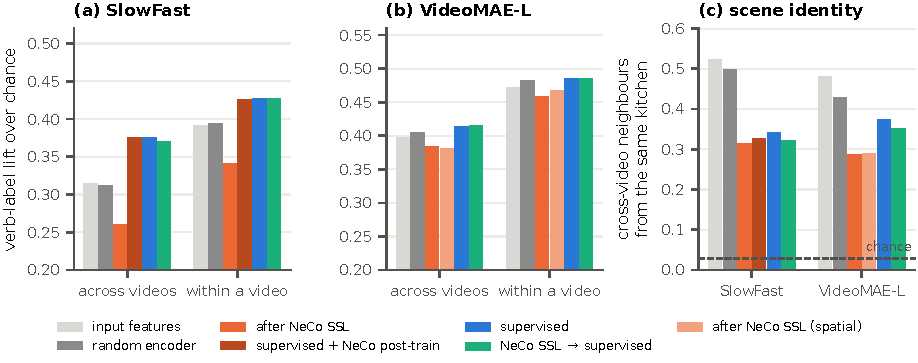
\includegraphics[width=\linewidth]{figs/fig_representation.pdf}
\caption{Neighbour-label probe on the validation split: how much more often than chance
a timestep's 10 nearest neighbours (level-0 encoder features) share its verb, for
neighbours from other videos and from the same video. NeCo SSL (orange) \emph{lowers} the
verb consistency below both the input features and the untrained encoder. Supervised
training raises it, and an SSL-initialised encoder ends exactly where a randomly
initialised one does after supervised training (green vs.\ blue). NeCo post-training of the
supervised encoder (dark orange) leaves its lift unchanged. \textbf{(c)} Kitchen probe:
fraction of cross-video neighbours from the same kitchen (chance 0.03). NeCo removes scene
identity rather than exploiting it.}
\label{fig:knn}
\end{figure}

If NeCo helped TAL the way it helps segmentation, it should make a timestep's nearest
neighbours more likely to share its verb, just as it makes VOC patches' neighbours share
their class (\cref{sec:voc}). \Cref{fig:knn} shows the opposite. On SlowFast, the input
features have a verb-label lift of 0.31 across videos and 0.39 within videos, and the
untrained encoder preserves this (0.31 / 0.39). After NeCo SSL the lift \emph{drops} to
0.26 / 0.34. VideoMAE-L shows the same direction with a smaller drop (0.41 / 0.48
$\rightarrow$ 0.38 / 0.46). Supervised training raises the lift to 0.38 / 0.43
(SlowFast). The objective is thus not merely neutral for TAL: it reorganises the encoder's
neighbourhoods \emph{against} the verb structure, both across videos and between
different actions within the same video, which is the distinction TAL depends on.
Post-training behaves differently. Applied to the supervised encoder (P2), NeCo leaves
the verb-label lift exactly where it was (0.375 / 0.426 vs.\ 0.375 / 0.427): starting from
an encoder that already groups verbs, a short, gentle update does not undo that grouping.
P2's $-1.34$\pp{} drop therefore does not come from lost verb structure. It comes from the
features moving relative to heads that were fitted to the old features and stay frozen.
A 0.87\% weight change is enough for that.

\subsection{No head start, and supervised training erases the SSL changes}\label{sec:why-erase}

The supervised loss confirms this from the downstream side. In seed-matched pairs, the
SSL-initialised model starts supervised training with a \emph{higher} loss than the
randomly initialised one: $+4.0\%$ and $+4.7\%$ over the first epoch on SlowFast (seeds 1,
2), and $+1.4\%$ on VideoMAE-L (\cref{fig:movement}b). Once supervised training starts,
the SSL changes disappear. The SSL-initialised encoder ends with the same verb-label lift
as the randomly initialised one (0.37 vs.\ 0.38 across videos, 0.43 vs.\ 0.43 within;
VideoMAE-L 0.42 vs.\ 0.41), and the two training curves coincide from epoch 10 on
(\cref{fig:trajectories}). The supervised schedule moves the encoder five times further
than SSL did, so it overwrites what SSL did instead of building on it. He et
al.~\cite{he2019rethinking} observed the same with full schedules for ImageNet
pre-training, but here not even the convergence-speed benefit remains, because the SSL
starting point is slightly worse.

\subsection{Objective or views? View identity and spatial crops}\label{sec:why-views}

\begin{figure}[t]
\centering
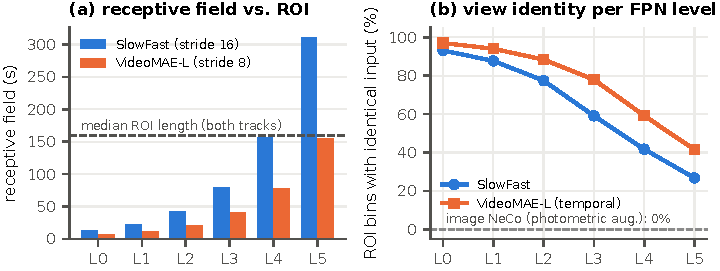
\includegraphics[width=0.78\linewidth]{figs/fig_views.pdf}
\caption{View identity under temporal cropping, computed by running the training crop
sampler on the true EPIC training-video lengths (40 crop pairs per video).
\textbf{(a)} Receptive field of each pyramid level in seconds, against the median ROI
length. \textbf{(b)} Fraction of ROI bins whose entire receptive field lies within
both crops, i.e.\ where the two views give the encoder identical input. In
image NeCo, colour jitter, blur and rescaling change every pixel, so this fraction is 0.}
\label{fig:views}
\end{figure}

In NeCo the objective is invariance to whatever distinguishes the two views, so the
views define what is learned~\cite{chen2020simclr,tian2020goodviews}. In image NeCo the
two views of a patch differ in scale, colour, blur and context. With pre-extracted clip
features, pixel-level augmentations are impossible, and temporal cropping changes only the
\emph{context} around a position, not the position's input. A ROI bin at position $p$ on
level $l$ receives identical input in both views whenever its receptive field
$[p-r_l,p+r_l]$ is cut identically by both crops. From the architecture, $r_l$ is 12, 21,
39, 75, 147 and 291 feature steps for levels 0--5. Running the actual crop sampler on the
true video lengths (\cref{fig:views}) shows that, for SlowFast, \textbf{93\% of level-0
bins and 77\% of level-2 bins see identical inputs in both views}. Only the coarsest
levels, whose receptive fields (up to 5\,min) exceed the median ROI ($\sim$160\,s), see
substantially different context. VideoMAE-L is even more extreme (97\% at level 0). This
is an upper bound on identical \emph{outputs}: at levels $\ge 1$ the two views' sampling
grids can be offset by a fraction of the stride, and stochastic depth adds noise.

With temporal crops, the only thing the student and teacher can disagree about is
therefore the distant context of a timestep. What NeCo teaches is invariance to that
context, which could flatten the differences between consecutive actions within a
video. Spatial crops remove this confound: the two views differ in their input at every
timestep, as image views do. If view identity were the cause, spatial crops should behave
differently. They do not. The objective is fit even better (top-1 agreement 0.96), the
encoder moves just as much (4.5\%), and the verb-label lift falls just as far: 0.38 across
videos (temporal crops: 0.38; untrained encoder: 0.41) and 0.47 within videos (temporal:
0.46; untrained: 0.48; \cref{fig:knn}b). Downstream mAP is 29.22 against 29.60. The
within-video drop is slightly smaller with spatial crops, so invariance to temporal context
may contribute a little, but the main effect does not depend on how the views are made.
The cause lies in what the objective asks of this representation, not in the
augmentations.

\subsection{Scene identity}\label{sec:why-scene}

NeCo ranks each anchor against references from \emph{other} videos. On VOC, object
classes recur across images, so a ranking that is consistent across views tends to
track semantics. EPIC videos differ most strongly by kitchen, and appearance cues such as
the counter and lighting are constant within a video and identical in both views. A
consistent ranking of other-video references could therefore be driven by scene
similarity, which is a nuisance for verbs shared across kitchens. The kitchen probe tests
this directly by asking whether cross-video neighbours come from the same kitchen more
often after SSL. The answer is no, and clearly so (\cref{fig:knn}c). For the input SlowFast
features, 52\% of a timestep's cross-video neighbours come from its own kitchen (chance:
3\%), and the untrained encoder keeps 50\%. After NeCo SSL this falls to 31\%, below even the
supervised encoder (34\%). VideoMAE-L shows the same pattern (0.48 input, 0.43 untrained,
0.29 after SSL with either view type, 0.37 supervised). NeCo therefore does not exploit scene
identity; it removes it. Supervised training also removes scene identity, but replaces it
with verb structure. NeCo removes scene and verb identity together, so its neighbourhoods
become less informative about both. One reading is that a ranking of references drawn from
other videos is most easily kept consistent by features that discard what distinguishes
one video, or one moment, from another. Whatever the mechanism, scene shortcuts are not
what makes NeCo fail here.

\subsection{Control: NeCo works in its own setting}\label{sec:voc}

\begin{figure}[t]
\centering
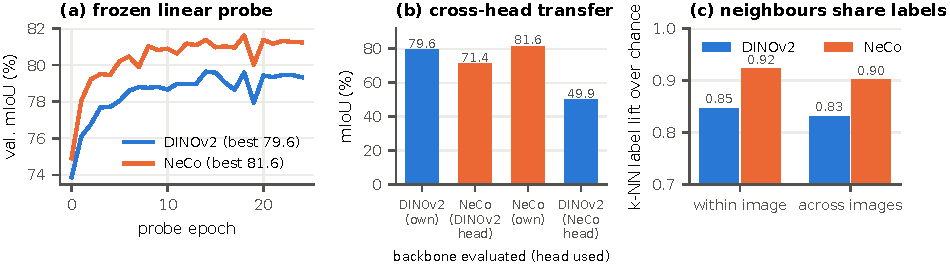
\includegraphics[width=\linewidth]{figs/fig_voc.pdf}
\caption{NeCo vs.\ DINOv2 (ViT-S/14) on PASCAL VOC 2012 under an identical, seed-matched
protocol. \textbf{(a)} Frozen-backbone linear probe: NeCo is ahead from the first epoch
and ends +2.0\,mIoU higher. \textbf{(b)} Neither trained head transfers to the other
backbone, so NeCo changes the representation itself rather than rescaling it. \textbf{(c)}
NeCo's $k$-NN neighbours (k=10) share the query patch's label more often, shown as lift
over the label-prior chance level.}
\label{fig:voc}
\end{figure}

If the NeCo objective were generically too far from downstream tasks, it would also fail
where it was designed to work. We test this with the official code and released weights:
NeCo-post-trained DINOv2 ViT-S/14 against the original DINOv2, evaluated on PASCAL VOC
2012~\cite{everingham2010voc} semantic segmentation with a frozen backbone and a
1$\times$1 linear head. Both runs use the same seed, head initialisation and data order.
NeCo reaches 81.6 mIoU against 79.6 (published: 81.4) and is ahead from the first epoch
(\cref{fig:voc}a). The representation itself changes (\cref{fig:voc}b), and in the
intended direction: NeCo's patch neighbours share the query's ground-truth label more
often, both within images (lift 0.92 vs.\ 0.85) and across images (0.90 vs.\ 0.83), and
k-means clusters align better with the classes (NMI 0.37 vs.\ 0.33).

\Cref{tab:contrast} sets the two settings side by side, using the same three probes. Every
probe has the opposite sign. On VOC, NeCo makes neighbours more label-consistent, starts
the downstream task with a lower loss, and improves the downstream metric. On EPIC it does
the reverse on the first two and nothing on the third. The objective is the same; what
differs is the setting it is applied to. In VOC, NeCo (1) refines a generic SSL backbone
that \emph{produces} the features, (2) on views that differ at every pixel, (3) against
references in which object classes recur across images. In our TAL setting, (1) the
features are frozen and already supervised for the target classes, and only a re-mixing
encoder is trained, (2) the temporal views are mostly identical inputs, and (3) the
references come from other kitchens. The spatial-crop and kitchen probes rule out (2)
and (3) as the main cause. Views that differ at every timestep give the same drop, and
NeCo removes scene identity rather than exploiting it. What remains is (1). On VOC, NeCo
sharpens a generic representation whose neighbourhoods already follow object classes.
Here it acts on features whose neighbourhoods are already organised by the target
verbs, and its target, a consistent ordering with respect to other videos, does not
coincide with that organisation, so meeting it costs verb structure.

\begin{table}[t]
\centering\small
\caption{The same probes in NeCo's own setting and in ours.}
\label{tab:contrast}
\begin{tabular}{lcc}
\toprule
Probe (NeCo vs.\ its start) & VOC (DINOv2) & EPIC: SlowFast / VideoMAE-L \\
\midrule
neighbour-label lift, across images/videos & $0.83\rightarrow0.90$ & $0.31\rightarrow0.26$ / $0.41\rightarrow0.38$ \\
neighbour-label lift, within image/video & $0.85\rightarrow0.92$ & $0.39\rightarrow0.34$ / $0.48\rightarrow0.46$ \\
first-epoch downstream loss & $-5\%$ (train), $-10\%$ (val) & $+4.0\%$, $+4.7\%$ / $+1.4\%$ \\
downstream metric & $+2.0$ mIoU & $+0.44$\pp{} (n.s.) / $+0.04$\pp{} \\
\bottomrule
\end{tabular}
\end{table}

%=======================================================================================
\section{Discussion}\label{sec:discussion}
%=======================================================================================

\paragraph{Putting it together.} The SSL stage behaves as an SSL stage should. It fits its
objective and moves the encoder by a fifth of what supervised training does. What it
learns from scratch, however, is a neighbourhood structure that is \emph{less} aligned with
verbs than the one the encoder starts with. As pre-training, this hands supervised training
a slightly worse starting point, which supervised training, moving the encoder five times
further, simply overwrites. As post-training, it leaves the verb grouping intact but
shifts the features under heads that cannot follow ($-1.34$\pp). In neither case does the
objective add anything the supervised signal lacks. The result is a null on two feature tracks. The neighbour-label probe
predicts this outcome cheaply: it needs no supervised run, and in both settings its sign
matches the downstream result.

\paragraph{Lessons for SSL on frozen-feature detectors.} \emph{First, check alignment
before the full pipeline.} A probe of whether the SSL representation brings same-label
units together costs minutes and anticipated every downstream result here, in both
directions. \emph{Second, better views are not enough.} Temporal crops of a pre-extracted
sequence differ only in distant context, but replacing them with views that differ
everywhere did not change the outcome. Whether an objective helps depends on how its target
relates to the representation it starts from, which is what the probe measures. \emph{Third, a single-seed baseline is not a reference.} The 1.4\pp{} seed
range of the SlowFast baseline exceeds every SSL effect we measured in pre-training.

\paragraph{Limitations.} Seed replicates exist only for the SlowFast P1/P3 comparison
($n{=}3$ each); VideoMAE-L and P2 are single runs. The neighbour-label probe uses level-0
features and $k{=}10$ only, and the view-identity analysis is computed from the
architecture rather than measured on activations. Only one dataset and one detector are
studied. We infer P2's head mismatch from the unchanged neighbour structure but do not
test whether briefly re-fitting the heads recovers the loss. We also do not test whether a
randomly perturbed initialisation of the same magnitude
as the SSL change would behave like the SSL initialisation. Since there is no gain to
explain, this control is not needed to support the negative result.

\paragraph{What would help instead.} Since information is fixed upstream, the lever is the
features. Switching from SlowFast to EPIC-finetuned VideoMAE-L gained 6.2\pp, against
$<$1\pp{} for any SSL variant. Promising directions are end-to-end or parameter-efficient
backbone adaptation for TAL~\cite{liu2024adatad}, and domain-adaptive self-supervised
pre-training of the \emph{backbone} on EPIC video, where pixel-level views are available and
NeCo's assumptions hold. Localization-aware pre-training objectives such as TSP and
BSP~\cite{alwassel2021tsp,xu2021bsp} are a third option. If SSL is applied to the TAL
encoder at all, the objective's neighbourhood alignment with the target labels should be
checked on the starting representation before any downstream training.

%=======================================================================================
\section{Conclusion}
%=======================================================================================

NeCo-style self-supervision of ActionFormer's encoder does not improve temporal action
localization on EPIC-KITCHENS-100 verbs. Post-training a converged model lowers average mAP
by 1.34\pp. Pre-training is indistinguishable from the baseline on SlowFast (three seeds)
and VideoMAE-L. The failure is not one of optimisation, since the objective is fit and the
encoder moves substantially. NeCo moves timestep neighbourhoods away from the verb structure,
gives supervised training a slightly worse starting point, and is overwritten by it. This
holds for views that differ at every timestep, and it is not a scene shortcut. In NeCo's own
dense-image setting the same probes all point the other way. The negative result
is therefore a statement about self-supervising a re-mixing encoder over frozen,
already-supervised clip features, not about neighbour-consistency learning in general.

\small
\bibliographystyle{unsrtnat}
\bibliography{refs}

\end{document}
